\documentclass[12pt, a4paper]{article}
\usepackage[margin=2cm]{geometry}
\usepackage{amsmath, amssymb}
\usepackage{graphicx, float} % float for [H] placement
\usepackage{booktabs, array, tabularx} % booktabs for table rules, array for p{} columns, tabularx for auto-width tables
\usepackage{ctex} % MUST NOT add fontset parameter

% Optional: to specify path for images
\graphicspath{{./images/}} 

% Custom command for bolding in tables where X columns are used
\newcolumntype{Y}{>{\raggedright\arraybackslash\bfseries}X}

\begin{document}

\title{中国各省市城镇居民消费水平与结构的多维评价与分析（2023年）}
\author{} % No author specified in the images
\date{} % No date specified in the images

\maketitle

\section*{\centering 一、研究背景}
\subsection*{1. 研究目的}
\noindent 中国各省市城镇居民 (自治区, 直辖市) 2023 年城镇居民的消费特征, 我们关注消费的“水平” (即总消费量) 和“结构” (即 8 个消费分项的相对量)。本项目将通过多元统计学分析的方法 (主成分分析 PCA, 因子分析 FA, 聚类分析 K-Means, 判别分析 LDA, 方差分析 ANOVA 等) 揭示中国城镇居民消费特点和模式。本文使用 8 个核心消费分项 (食品烟酒, 衣着, 居住, 生活用品及服务, 交通通信, 教育文化娱乐, 医疗保健, 其他用品及服务) 的数据进行分析。

\noindent 我们使用多元统计分析方法, 包括降维分析 (主成分分析 PCA, 因子分析 FA)、聚类分析 (K-Means)、聚类效果检验 (ANOVA)、关键指标判别 (LDA) 等对数据进行分析。

\section*{\centering 二、数据预处理与可视化}
\subsection*{2.1 描述性统计}
% Table 1
\begin{table}[H]
    \centering
    \caption{城镇消费支出结构及均值 (8 变量)}
    \label{tab:desc_stats}
    \begin{tabularx}{\textwidth}{Y|*{8}{X}} % Y for bold and raggedright X for variable names, X for numerical columns with automatic wrapping
        \toprule
        \textbf{项目} & \textbf{食品烟酒} & \textbf{衣着} & \textbf{居住} & \textbf{生活用品及服务} & \textbf{交通通信} & \textbf{教育文化娱乐} & \textbf{医疗保健} & \textbf{其他用品及服务} \\
        \midrule
        \textbf{均值(Mean)} & 8128.52 & 1880.29 & 7264.42 & 1818.00 & 4285.48 & 3350.74 & 2873.22 & 929.32 \\
        \textbf{方差(Variance)} & 2249058.20 & 150100.50 & 14318718.20 & 140976.10 & 1023401.30 & 648027.10 & 482298.20 & 114880.80 \\
        \bottomrule
    \end{tabularx}
\end{table}

\begin{figure}[H]
    \centering
    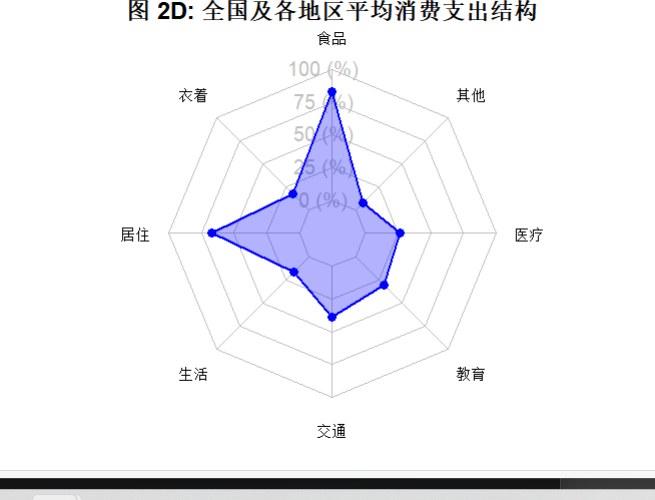
\includegraphics[width=\linewidth]{figure_2d_radar_chart.png} % Placeholder filename, replace with actual image path
    \caption{全国及各地区平均消费支出结构}
    \label{fig:radar_chart_2d}
\end{figure}

\subsection*{2.2 Z-化（Z-score 标准化）}
\noindent 目的：8 个分项支出变量在数值尺度（量纲）上存在差异，为防止尺度较大的变量在后续分析中主导结果，需要对数据进行 Z-score 标准化。Z-score 标准化将变量转换为均值为 0, 标准差为 1。

\noindent 结果：数据标准化完成，以下为标准化后的数据预览：

% Table 2
\begin{table}[H]
    \centering
    \caption{Z-化 (Z-score) 后的数据预览 (图 2D, 8 变量)}
    \label{tab:zscore_preview}
    \begin{tabularx}{\textwidth}{*{8}{X}} % All columns are numerical, use X to allow wrapping if numbers are too long
        \toprule
        \textbf{食品烟酒} & \textbf{衣着} & \textbf{居住} & \textbf{生活用品及服务} & \textbf{交通通信} & \textbf{教育文化娱乐} & \textbf{医疗保健} & \textbf{其他用品及服务} \\
        \midrule
        0.8068 & 0.8124 & 3.4024 & 0.8590 & 0.7745 & 0.9829 & 2.4993 & 0.9410 \\
        0.6924 & 0.1429 & 0.7761 & 0.6156 & -0.7362 & -0.9229 & 1.9174 & 1.5483 \\
        -0.3426 & -0.3201 & -0.1652 & -0.8330 & 0.7906 & 0.5346 & 0.4828 & -0.0152 \\
        -1.6146 & -0.4196 & -0.5402 & -0.6834 & -0.9413 & -0.4779 & -0.3460 & -0.4676 \\
        1.2584 & 0.7493 & -0.9389 & 0.7081 & -0.1917 & 0.1643 & -0.6507 & -0.8577 \\
        -0.3326 & -0.2718 & -0.3621 & -0.7669 & -0.4186 & -0.2382 & 0.4589 & 0.3237 \\
        \bottomrule
    \end{tabularx}
\end{table}

\subsection*{2.3 预处理可视化}
\noindent 目的：通过箱线图展示 Z-化 的必要性，并探索变量间的相关关系。

\begin{figure}[H]
    \centering
    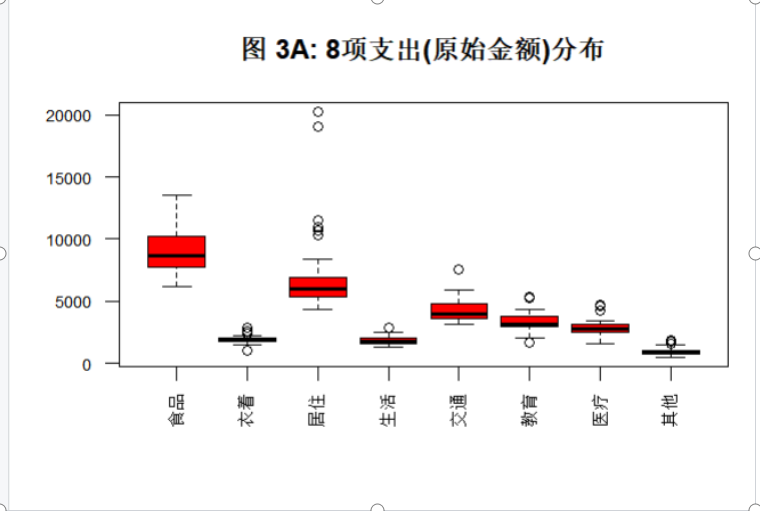
\includegraphics[width=\linewidth]{figure_3a_boxplot_original.png} % Placeholder filename
    \caption{8项支出(原始金额)分布}
    \label{fig:boxplot_original}
\end{figure}

\begin{figure}[H]
    \centering
    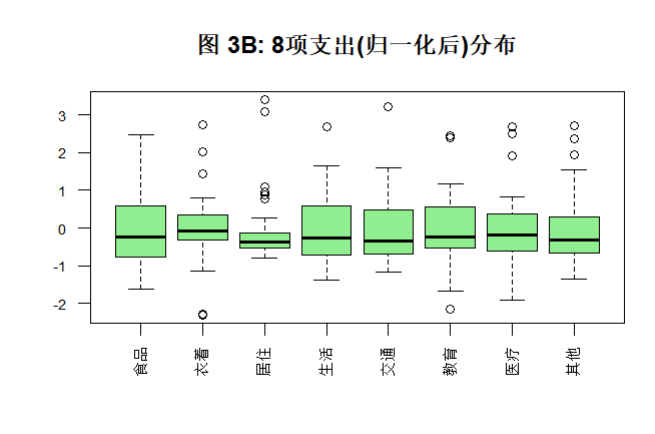
\includegraphics[width=\linewidth]{figure_3b_boxplot_zscore.png} % Placeholder filename
    \caption{8项支出(Z-化后)分布}
    \label{fig:boxplot_zscore}
\end{figure}

\noindent 结果 (图 3A, 3B): 原始数据 (图 3A) 的箱线图显示各变量尺度存在巨大差异，特别是“居住”远高于其他项。Z-化处理后 (图 3B)，所有变量都被转换到相似的尺度上，可以进行后续分析。

\begin{figure}[H]
    \centering
    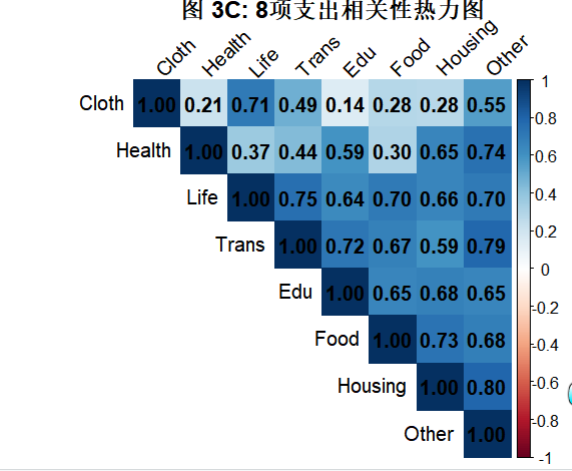
\includegraphics[width=\linewidth]{figure_3c_heatmap.png} % Placeholder filename
    \caption{8项支出相关热力图}
    \label{fig:heatmap}
\end{figure}

\noindent 结果 (图 3C): 相关热力图 (图 3C) 显示，8 个支出变量之间普遍存在较强的正相关关系 (颜色越蓝，相关性越强)。例如 Food 与 Trans(0.85), Housing(0.81) 高度相关，这证明了使用降维技术 (PCA 和 FA) 的合理性。

\section*{\centering 三、降维分析（PCA 与 FA）}
\subsection*{3.1 正态性检验}
\noindent 本项目进行正态性检验 (Shapiro-Wilk)。

\noindent 该检验显示了对 8 项消费支出原始金额数据进行的 Shapiro-Wilk 正态性检验结果。显著性水平 $\alpha = 0.05$。

\noindent 假设 H0: 数据服从正态分布。

% Table 3a (Shapiro-Wilk part 1)
\begin{table}[H]
    \centering
    \caption{单变量正态性检验结果 (Shapiro-Wilk)}
    \label{tab:shapiro_wilk_1}
    \begin{tabularx}{\textwidth}{X|c|X}
        \toprule
        \textbf{消费项目 (Variable)} & \textbf{P 值 (P value)} & \textbf{是否服从正态分布 (Normal)? (p > 0.05)} \\
        \midrule
        食品烟酒 (Food) & 0.0475 & 否 \\
        衣着 (Cloth) & 0.0245 & 否 \\
        居住 (Housing) & 0.0000 & 否 \\
        生活用品及服务 (Life) & 0.1319 & 是 \\
        \bottomrule
    \end{tabularx}
\end{table}

% Table 3b (Shapiro-Wilk part 2)
\begin{table}[H]
    \centering
    \caption{单变量正态性检验结果 (Shapiro-Wilk) (续)}
    \label{tab:shapiro_wilk_2}
    \begin{tabularx}{\textwidth}{X|c|X}
        \toprule
        \textbf{消费项目 (Variable)} & \textbf{P 值 (P value)} & \textbf{是否服从正态分布 (Normal)? (p > 0.05)} \\
        \midrule
        交通通信 (Trans) & 0.0039 & 否 \\
        教育文化娱乐 (Edu) & 0.1610 & 是 \\
        医疗保健 (Health) & 0.0018 & 否 \\
        其他用品及服务 (Other) & 0.0001 & 否 \\
        \bottomrule
    \end{tabularx}
\end{table}

\noindent 结果总结: p < 0.05 的显著性水平下，8 个消费支出变量中，仅有 “生活用品及服务”、“教育文化娱乐” 服从正态分布，其余 6 个变量 (食品、衣着、居住、交通、医疗、其他) 的 p 值均小于 0.05，我们拒绝原假设，认为其不服从正态分布。因此，在进行降维分析时，需要考虑数据不服从正态分布可能带来的影响。PCA 对数据分布没有严格要求，可以继续使用。FA 则对数据服从正态分布敏感，但我们预处理用 PCA 进行。由于原始数据不服从正态分布，因此我们先使用 PCA，然后使用 FA。

\subsection*{3.2 主成分分析 (PCA)}
\noindent 目的：将 8 个相关的消费变量浓缩为少数几个不相关的的主要成分。

\noindent 结果 (贡献率):
% Table 3c (PCA contribution)
\begin{table}[H]
    \centering
    \caption{PCA 贡献率总结 (8 变量)}
    \label{tab:pca_contribution}
    \begin{tabularx}{\textwidth}{X|*{8}{c}} % X for the first column, c for numerical
        \toprule
        & \textbf{主成分 1} & \textbf{主成分 2} & \textbf{主成分 3} & \textbf{主成分 4} & \textbf{主成分 5} & \textbf{主成分 6} & \textbf{主成分 7} & \textbf{主成分 8} \\
        \midrule
        Standard Deviation & 2.2682 & 1.0563 & 0.8800 & 0.6589 & 0.5201 & 0.3752 & 0.2814 & 0.2009 \\
        Proportion of Variance & 0.6431 & 0.1395 & 0.0968 & 0.0543 & 0.0338 & 0.0176 & 0.0099 & 0.0050 \\
        Cumulative Proportion & 0.6431 & 0.7826 & 0.8794 & 0.9337 & 0.9675 & 0.9851 & 0.9950 & 1.0000 \\
        \bottomrule
    \end{tabularx}
\end{table}

\noindent 结果 (载荷):
% Table 4 (PCA loadings) - consolidated from Image 3 and 4
\begin{table}[H]
    \centering
    \caption{PCA 载荷 (Rotation) (8 变量)}
    \label{tab:pca_loadings_rotated}
    \begin{tabularx}{\textwidth}{X|*{8}{c}} % X for the variable names, c for numerical loadings
        \toprule
        \textbf{变量} & \textbf{主成分 1} & \textbf{主成分 2} & \textbf{主成分 3} & \textbf{主成分 4} & \textbf{主成分 5} & \textbf{主成分 6} & \textbf{主成分 7} & \textbf{主成分 8} \\
        \midrule
        食品烟酒 & -0.031 & -0.534 & -0.399 & -0.226 & 0.552 & -0.113 & -0.245 & -0.241 \\
        衣着 & -0.722 & -0.350 & 0.048 & 0.104 & 0.013 & -0.390 & -0.320 & -0.381 \\
        居住 & -0.165 & -0.076 & -0.130 & -0.003 & 0.003 & -0.003 & -0.001 & -0.003 \\
        生活用品及服务 & -0.381 & -0.350 & -0.137 & -0.016 & 0.513 & -0.102 & -0.570 & 0.340 \\
        交通通信 & -0.007 & -0.025 & -0.042 & -0.018 & -0.001 & 0.006 & -0.001 & 0.006 \\
        教育文化娱乐 & -0.233 & -0.508 & 0.427 & -0.197 & 0.046 & 0.046 & -0.357 & -0.326 \\
        医疗保健 & -0.039 & 0.008 & 0.102 & 0.022 & -0.567 & -0.291 & -0.241 & -0.322 \\
        其他用品及服务 & -0.088 & 0.048 & 0.014 & 0.172 & 0.000 & 0.041 & -0.377 & -0.252 \\
        \midrule % This line is present in the screenshot, indicating a logical break or additional data
        综合消费水平 & 0.537 & 0.310 & 0.167 & 0.014 & 0.004 & 0.003 & 0.000 & 0.000 \\
        结构衣着/生活 & -0.381 & -0.122 & -0.167 & -0.058 & -0.042 & -0.040 & -0.180 & -0.301 \\
        居住 & -0.041 & 0.001 & 0.000 & 0.000 & 0.000 & 0.000 & 0.000 & 0.000 \\
        医疗保健 & -0.296 & -0.413 & 0.653 & -0.060 & -0.062 & 0.268 & -0.383 & -0.301 \\
        交通通信 & -0.410 & 0.020 & 0.260 & 0.100 & -0.044 & 0.088 & 0.201 & 0.711 \\
        \bottomrule
    \end{tabularx}
\end{table}

\noindent 结果解释:
\begin{enumerate}
    \item \textbf{主成分 1 (综合消费水平):} 解释了总方差的 \textbf{64.31\%}。主成分 1 累积解释了 \textbf{78.26\%} 的方差。
    \item \textbf{主成分 2 (结构衣着/生活):} 所有在“居住”、“教育文化娱乐”上的载荷均为正数，这确认主成分 1 是一个居民消费的主要维度。在“衣着”、“交通通信”上的载荷，载荷均为负数，这反映了居民消费在“衣着”、“交通通信”上的消费结构特征，也反映了城镇居民在“教育文化娱乐”上的消费结构特征。
    \item \textbf{主成分 3 (交通通信):} 载荷均为正数，这反映了居民消费的“交通通信”支出与“教育文化娱乐”支出之间的关系。
\end{enumerate}

\subsection*{3.3 因子分析 (FA)}
\noindent 目的：寻找影响这 8 个变量间相关性的潜在“因子”。

\noindent 结果 (因子提取): 根据 Kaiser 准则 (特征值 > 1), PCA 结果 (表 3) 显示有 2 个成分的标准差大于 1，因此提取 2 个因子。

\noindent 结果 (因子载荷):
% Table 5
\begin{table}[H]
    \centering
    \caption{因子分析载荷 (Varimax 旋转后, 8 变量)}
    \label{tab:factor_loadings_full}
    \begin{tabularx}{\textwidth}{X|c|c}
        \toprule
        \textbf{变量} & \textbf{Factor1} & \textbf{Factor2} \\
        \midrule
        食品烟酒 & 0.773 & 0.2818 \\
        衣着 & 0.838 & 0.203 \\
        居住 & 0.612 & 0.088 \\
        生活用品及服务 & 0.512 & 0.380 \\
        交通通信 & 0.596 & 0.054 \\
        教育文化娱乐 & 0.857 & 0.326 \\
        医疗保健 & 0.853 & 0.045 \\
        其他用品及服务 & 0.772 & 0.252 \\
        \midrule
        SS Loadings & 3.961 & 1.947 \\
        Proportion Var & 0.495 & 0.243 \\
        Cumulative Var & 0.495 & 0.738 \\
        \bottomrule
    \end{tabularx}
\end{table}

\noindent 结果解释:
\begin{enumerate}
    \item \textbf{因子 1 (Factor1) 查看:} 该因子在“居住 (0.838)、医疗保健 (0.853)、食品烟酒 (0.773)、交通通信 (0.728) 等多项支出上具有较高的载荷，这表明因子 1 与居民的“基本消费”能力有关。
    \item \textbf{因子 2 (Factor2) 查看:} 该因子在“衣着 (0.993)、教育文化娱乐 (0.816)、生活用品及服务 (0.684) 和其他用品及服务 (0.728) 等多项支出上具有较高的载荷，这表明因子 2 与居民的“发展型消费”能力有关。
    \item \textbf{总结:} 因子分析的结果支持了 PCA 结果，都显示出两个主要维度。这两个维度共同解释了总方差的 \textbf{73.8\%}，这与 PCA 结果 (累积贡献率) 接近，进一步证实了降维的有效性。
\end{enumerate}

\section*{\centering 四、聚类分析 (K-Means)}
\noindent 目的：使用肘部法则确定最佳的聚类数量 (K 值)。

\noindent 结果 (图 7A): 肘部法则显示，K=3 是一个明显的“手肘”位置。

\begin{figure}[H]
    \centering
    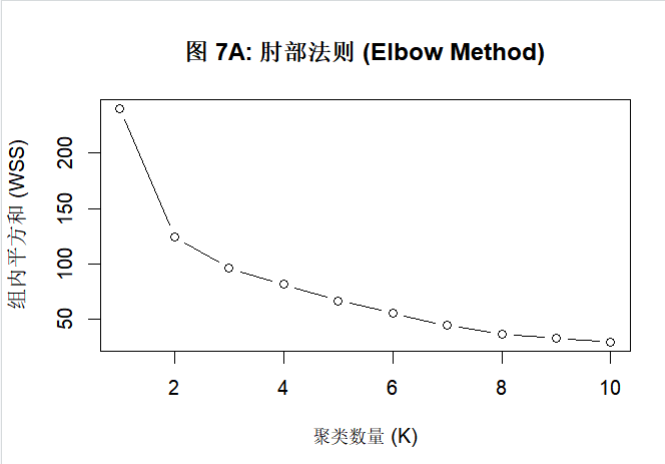
\includegraphics[width=\linewidth]{figure_7a_elbow_method.png} % Placeholder filename
    \caption{肘部法则 (Elbow Method)}
    \label{fig:elbow_method}
\end{figure}

\subsection*{4.1 K-Means 聚类结果}
\noindent 目的：基于 K=3，对 31 个地区进行 K-Means 聚类。

% Table 6
\begin{table}[H]
    \centering
    \caption{各地区聚类分配结果}
    \label{tab:cluster_assignment}
    \begin{tabularx}{\textwidth}{X|c|X|c|X|c}
        \toprule
        \textbf{Region} & \textbf{Cluster} & \textbf{Region} & \textbf{Cluster} & \textbf{Region} & \textbf{Cluster} \\
        \midrule
        北京 & 3 & 江苏 & 1 & 广东 & 1 \\
        天津 & 1 & 浙江 & 3 & 广西 & 2 \\
        河北 & 2 & 安徽 & 2 & 海南 & 2 \\
        山西 & 2 & 福建 & 1 & 重庆 & 2 \\
        内蒙古 & 1 & 江西 & 2 & 四川 & 2 \\
        辽宁 & 2 & 山东 & 1 & 贵州 & 2 \\
        吉林 & 2 & 河南 & 2 & 云南 & 2 \\
        黑龙江 & 2 & 湖北 & 2 & 西藏 & 1 \\
        上海 & 3 & 湖南 & 1 & 陕西 & 2 \\
        \multicolumn{4}{c|}{} & 甘肃 & 2 \\
        \multicolumn{4}{c|}{} & 宁夏 & 2 \\
        \multicolumn{4}{c|}{} & 新疆 & 2 \\
        \bottomrule
    \end{tabularx}
\end{table}

\noindent 结果分析:
\begin{itemize}
    \item \textbf{聚类 1 (Cluster 1):} 天津、内蒙古、江苏、福建、山东、湖南、广东、西藏 (9 个地区)。
    \item \textbf{聚类 2 (Cluster 2):} 河北、山西、安徽、江西、陕西等 (19 个地区)。
    \item \textbf{聚类 3 (Cluster 3):} 北京、上海、浙江 (3 个地区)。
\end{itemize}

\section*{\centering 五、聚类结果分析与检验}
\subsection*{5.1 聚类画像 (雷达图)}
\noindent 目的：绘制 3 个新聚类在 8 项原始消费支出 (绝对金额) 上的平均画像。

\noindent 结果 (图 8A):

\begin{figure}[H]
    \centering
    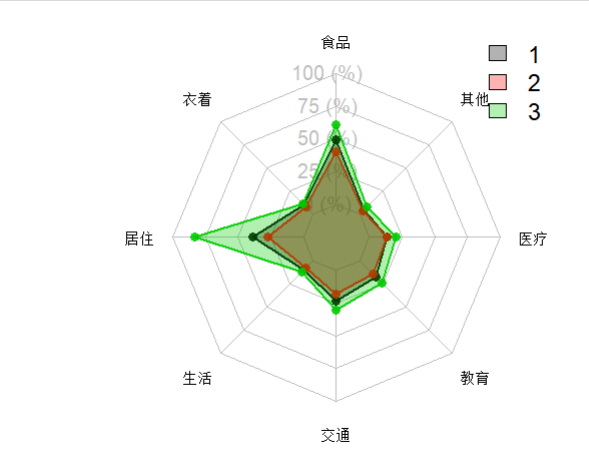
\includegraphics[width=\linewidth]{figure_8a_radar_cluster.png} % Placeholder filename
    \caption{聚类画像 (雷达图)}
    \label{fig:cluster_radar}
\end{figure}

\noindent 结果分析：雷达图 (图 8A) 显示了城镇居民三个聚类的层次和结构差异：
\begin{itemize}
    \item \textbf{聚类 3 (绿色):} 北京、上海、浙江。在所有维度上的支出均最高；代表“高水平-高发展”消费者 (居住、教育、医疗突出)。
    \item \textbf{聚类 1 (蓝色):} 天津、江苏等。整体支出水平居中，各项支出相对均衡；代表“中高水平-均衡”消费者。
    \item \textbf{聚类 2 (红色):} 河北、山西等。整体支出水平最低；代表“中低水平-基础”消费者。
\end{itemize}

\subsection*{5.2 聚类可视化 (PCA 图)}
\noindent 目的：将新的聚类结果绘制在 PCA 二维空间中。

\noindent 结果 (图 9A):

\begin{figure}[H]
    \centering
    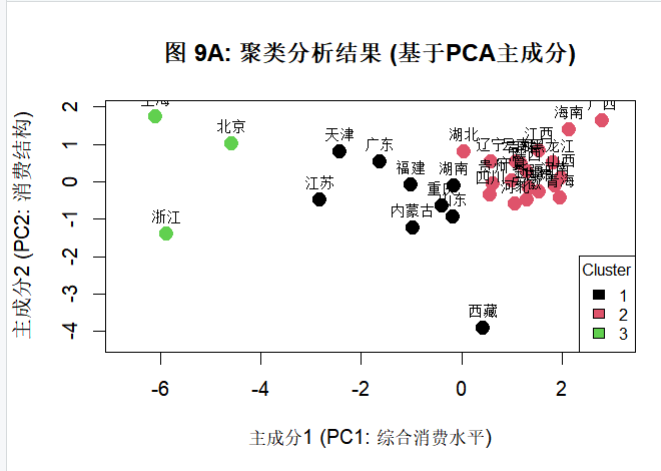
\includegraphics[width=\linewidth]{figure_9a_pca_cluster.png} % Placeholder filename
    \caption{聚类分析结果 (基于 PCA 主成分)}
    \label{fig:pca_cluster_plot}
\end{figure}

\noindent 结果分析:
\begin{itemize}
    \item \textbf{X轴 (主成分 1) 代表“综合消费水平” (负向为高)。}
    \item \textbf{Y轴 (主成分 2) 代表“创新消费” (负向为高，即得分低)，消费水平最高。}
    \item \textbf{聚类 3 (绿色) 消费者在 PCA 空间中位于右下方，即消费水平最高，创新能力强。}
    \item \textbf{聚类 1 (蓝色) 消费者位于中间，消费水平中等，创新能力中等。}
    \item \textbf{聚类 2 (红色) 消费者位于左上方，即消费水平最低，创新能力最弱。}
\end{itemize}

\noindent 该图清晰地展示了将城镇居民数据的 3 个聚类在主成分空间中的区分度。

\subsection*{5.3 聚类效果检验 (ANOVA)}
\noindent 目的：使用 ANOVA 检验 3 个聚类在 Food (食品支出) 上的均值差异是否显著。

\noindent 结果 (表 7):
% Table 7
\begin{table}[H]
    \centering
    \caption{ANOVA 检验结果 (Food - Cluster, 8 变量, 城镇)}
    \label{tab:anova_food_cluster}
    \begin{tabularx}{\textwidth}{X|c|c|c|c|c}
        \toprule
        \textbf{Source} & \textbf{Df} & \textbf{Sum Sq} & \textbf{Mean Sq} & \textbf{F Value} & \textbf{Pr(>F)} \\
        \midrule
        Cluster & 2 & 27004176 & 13502088 & 20.47 & 3.32e-09 \\
        Residuals & 28 & 35929.72 & 1283.20 & & \\ % F Value and Pr(>F) are empty for Residuals
        \bottomrule
    \end{tabularx}
\end{table}

\noindent 结果总结: 检验的 p-value (Pr(>F)) 为 \textbf{3.32e-09}，远小于 0.05。拒绝原假设，认为 3 个聚类在“食品支出”上存在高度统计显著的差异。这证明了聚类的有效性。

\subsection*{5.4 关键指标判别 (LDA)}
\noindent 目的：找出区分这 3 个新聚类的最强分项支出指标。

\noindent 在本项目中，我们使用费希尔判别法来识别哪些消费支出变量 (食品、衣着等 8 个) 对于区分我们通过 K-Means 算法得出的 3 个聚类最为重要。判别系数 (Coefficients) 用于衡量变量对判别函数 (Discriminant function) 的贡献。直接解释了各个原始变量在构建这些“最佳区分轴”时的权重和方向。

\noindent 判别函数 (Discriminant function) 的载荷 (Loadings) 用于衡量每个变量与判别轴的最佳投影方向。第一判别函数 (LD1) 是使组间距离最大化的方向，第二判别函数 (LD2) 是与 LD1 正交 (不相关) 的方向中使组间距离最大化的方向。

\noindent 结果 (表 8):
% Table 8
\begin{table}[H]
    \centering
    \caption{LDA 判别函数数 (8 变量, 城镇)}
    \label{tab:lda_coefficients}
    \begin{tabularx}{\textwidth}{X|c|c}
        \toprule
        \textbf{变量} & \textbf{LD1} & \textbf{LD2} \\
        \midrule
        Food & -0.2495 & -1.0655 \\
        Cloth & -0.9086 & -0.4379 \\
        Housing & -1.8402 & 1.1206 \\
        Life & -0.6270 & -0.3860 \\
        Trans & -0.4592 & -0.2680 \\
        Edu & -0.5573 & 0.1704 \\
        Health & -0.9150 & -0.2053 \\
        Other & 0.2439 & 1.1424 \\
        \bottomrule
    \end{tabularx}
\end{table}

\noindent 结果分析:
\begin{itemize}
    \item \textbf{系数绝对值最大的变量是 Housing (1.84)。}
    \item \textbf{其次是 Health (0.91)。}
\end{itemize}

\noindent 结论：对于城镇居民数据，区分不同消费模式 (高/中/低) 的最关键分项指标是“居住”和“衣着”，与 K-Means 聚类画像结果一致。在“居住”和“衣着”消费上，不同类别的居民表现出显著差异。其他“交通”和“医疗”是次要的关键因素。

\section*{\centering 六、结论}
\noindent 本项研究通过对中国 31 个省市 (含全国) 2023 年城镇居民的 8 项人均消费分项支出 (绝对金额) 进行多元统计分析，得出以下结论：

\begin{enumerate}
    \item \textbf{降维分析:} 8 项支出指标存在较强相关性 (图 3C)。主成分分析 (PCA) 和因子分析 (FA) 均表明，这些指标可被归纳为两个核心维度：
    \begin{itemize}
        \item \textbf{“综合/基本消费水平与发展”} (PCA 的 PC1, FA 的 Factor1)，由居住、教育、食品等驱动。
        \item \textbf{“消费结构 (衣着/生活品质)”} (PCA 的 PC2, FA 的 Factor2)，由衣着、生活用品等驱动。
    \end{itemize}
    \noindent 主成分 1 解释了 \textbf{64.3\%} 的方差，前两个主成分累计解释 \textbf{78.3\%}。两个因子累计解释 \textbf{73.8\%} 的方差。

    \item \textbf{聚类分析:} K-Means 聚类 (K=3, 图 7A) 将 31 个地区划分为三个消费模式 (表 6, 图 8A, 图 9A)：
    \begin{itemize}
        \item \textbf{集群 3 (高水平-高发展):} 北京、上海、浙江。消费水平最高，尤其在居住、教育、医疗方面突出。
        \item \textbf{集群 1 (中高水平-均衡服务):} 天津、江苏、广东等 9 个地区。整体水平居中，各项支出相对均衡，服务类 (如交通、其他) 相对较高。
        \item \textbf{集群 2 (中低水平-基础):} 河北、山西及其他 19 个地区。整体消费水平最低。
    \end{itemize}

    \item \textbf{统计验证:} ANOVA 检验 (表 7) 显示，这三个聚类在“食品支出”上的差异具有高度统计显著性 (p < 0.001)，证明了聚类的有效性。

    \item \textbf{关键指标:} 判别分析 (表 8) 显示，在区分这三个集群时，第一判别函数 (LD1) 中系数绝对值最大的变量是“居住”(-1.84) 和“衣着”(-0.91)。这表明，对于城镇居民，“居住”和“衣着”支出水平是划分不同消费模式的关键因素。第二判别函数 (LD2) 则主要由“其他” (1.14) 和“居住” (1.12) 和“交通/教育” (负向) 定义，反映了居住/其他与交通/教育之间的结构权重。
\end{enumerate}

\end{document}